% *********************************************************************
% © 2010–2022 Jeremy Sylvestre
%
% Permission is granted to copy, distribute and/or modify this document
% under the terms of the GNU Free Documentation License, Version 1.3 or
% any later version published by the Free Software Foundation; with no
% Invariant Sections, no Front-Cover Texts, and no Back-Cover Texts. A
% copy of the license is included in the appendix entitled “GNU Free
% Documentation License” that appears in the output document of this
% PreTeXt source code. All trademarks™ are the registered® marks of
% their respective owners.
%
% *********************************************************************

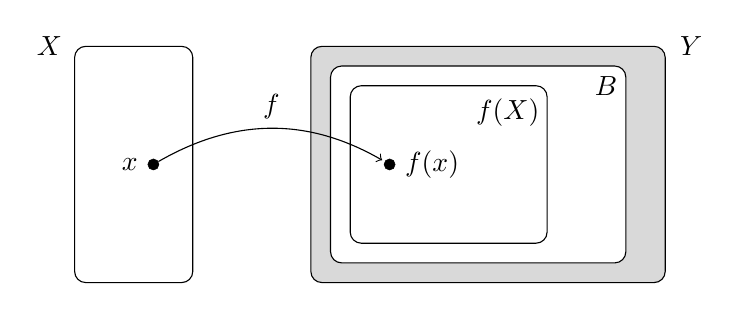
\begin{tikzpicture}[
	vertex/.style={ circle, draw, very thin, fill, inner sep=0pt, minimum size=4pt },
	vertexg/.style={ black!40!white, circle, draw, very thin, fill, inner sep=0pt, minimum size=4pt },
	vertexo/.style={ circle, draw, very thin, inner sep=0pt, minimum size=4pt }
]

\draw[rounded corners]
  (-2.5,-1.5) rectangle (-1,1.5);
\node at (-2.82,1.5) {$X$};
\draw[rounded corners,fill=black!15!white]
  (0.5,-1.5) rectangle (5,1.5);
\node at (5.33,1.5) {$Y$};
\draw[rounded corners,fill=white]
  (0.75,-1.25) rectangle (4.5,1.25);
\node at (4.25,1) {$B$};
\draw[rounded corners]
  (1,-1) rectangle (3.5,1);
\node at (3,0.66) {$f(X)$};
\node at (-1.5,0) (x) [vertex,label=left:{$x$}] {};
\node at (1.5,0) (y) [vertex,label=right:{$f(x)$}] {};
\draw[->,shorten >=1pt] (x) to [out=30,in=150] node[above] {$f$} (y);

\end{tikzpicture}
